\documentclass[10pt, a4paper, twoside]{article}

% Set up the standard margins for the document
% 42.2 left & 15.5 right is same as Forsling, Neymark
% 21.3 top  & 20 bottom is same as Olofsson
\usepackage[left=19.5mm, right=19.5mm, top=21.3mm, bottom=20mm]{geometry}

% Input file character encoding (kinda useless if we don't
% use åäö and stuff, but it doesn't hurt to have it)
\usepackage[utf8]{inputenc}
%\usepackage[swedish]{babel}

% Block Comments
\usepackage{comment}

% No indentation in new paragraph
\usepackage{parskip}

% To include graphics
\usepackage{graphicx}

% More mathematical symbols and fonts
\usepackage{amsmath}
\usepackage{amsfonts}
\usepackage{amssymb}

% Simple list
\usepackage[ampersand]{easylist}
\ListProperties(Hide=100, Hang=true, Progressive=5ex, Style*=$\bullet$ ,
Style2*=-- ,Style3*=$\circ$ ,Style4*=\tiny$\blacksquare$ )


% Clickable internal links
\usepackage{hyperref}
\usepackage[all]{hypcap} % without this the link takes you to the caption, not the top of the image
\hypersetup{ % Settings for links in documnet
	setpagesize = false, % Don't allow hyperref to change page size. Tips från Micke Olofsson
	colorlinks = true,   % No boxes around links
	linkcolor = black,citecolor = black,filecolor = black,urlcolor = black, % don't color links
}

% To include to first page pdf file
\usepackage{pdfpages}

% Add section number to equation and figure number (ex: 5.11 instead of simply 11)
\numberwithin{equation}{subsection}
\numberwithin{figure}{section}
\numberwithin{table}{section}

% Show program code listings in document
\usepackage{listings}

%
% Header stuff
%
\usepackage{fancyhdr}
\setlength{\headheight}{15pt}

\fancyhf{}
\fancyhead[LE, RO]{\thepage}
\fancyhead[RE]{TSBB15 2013: User's Manual}
\fancyhead[LO]{Object Tracking in Image Sequences}

\fancypagestyle{plain}{ %
\fancyhf{} % remove everything
\renewcommand{\headrulewidth}{0pt} % remove lines as well
\renewcommand{\footrulewidth}{0pt}}
%
% End header stuff
%




\begin{document}

% First page

\includepdf{Cover/cover.pdf}


% Project identity page
\newpage
\pagestyle{fancy}
\pagenumbering{roman}
\setcounter{page}{2} % sets the current page number to 2 

\begin{center}
    \vspace*{4\baselineskip}

	\textbf{\huge Project Kitchen Occupation} \\
	\vspace*{0.5\baselineskip}
	Bilder och Grafik CDIO, HT 2013 \\
	Department of Electrical Engineering (ISY), Link\"{o}ping University
	
	\vspace*{2\baselineskip}
	\textbf{\LARGE Participants}


	{\footnotesize 
	\begin{tabular}{|p{2.7cm}|p{1cm}|p{5cm}|p{2cm}|p{3.4cm}|}
		\hline
		\textbf{Name} & \textbf{Tag} & \textbf{Responsibilities} & \textbf{Phone} & \textbf{E-mail} \\
		\hline
		Mattias Tiger & MT & Project manager & 073--695\,71\,53 & matti166@student.liu.se \\
		\hline
		Erik Fall & EF & -- & 076--186\,98\,84 & erifa226@student.liu.se \\
		\hline
		Gustav Häger & GH & System integration & 070--649\,03\,97 & gusha124@student.liu.se \\
		\hline
		Malin Rudin & MR & -- & 073--800\,35\,77 & malru103@student.liu.se \\
		\hline
		Alexander Sjöholm & AS & -- & 076--225\,11\,74 & alesj050@student.liu.se \\
		\hline
		Martin Svensson & MS & Documentation & 070--289\,01\,49 & marsv106@student.liu.se \\
		\hline
		Nikolaus West & NW & Testing & 073--698\,92\,60 & nikwe491@student.liu.se \\
		\hline
	\end{tabular}
	}

{\footnotesize 
\vspace{0.5\baselineskip}
\textbf{Homepage}: TBA \\
\vspace{1\baselineskip}

\textbf{Customer}: Joakim Nejdeby, Link\"{o}ping University, Origo 3154 \\
\textbf{Customer contact}: 013--28\,17\,57, joakim.nejdeby@liu.se \\
\textbf{Project supervisor}: Fahad Khan, Link\"{o}ping University, fahad.khan@liu.se \\
\textbf{Examiner}: Michael Felsberg, michael.felsberg@liu.se \\
}

\end{center}



% table of contents
\newpage
\tableofcontents
\listoffigures
\listoftables

% list of figures
%\newpage
%\listoffigures


% Document history page
\newpage
\vspace*{5\baselineskip}

\begin{center}
\textbf{\LARGE Document history}

{ \footnotesize 
\begin{tabular}{|p{1cm}|p{2.0cm}|p{5cm}|p{1.5cm}|p{2cm}|}
	\hline

	\textbf{Version} & \textbf{Date} & \textbf{Changes} & \textbf{Sign} & \textbf{Reviewed} \\
	
	\hline
	0.1 & 2013--12--13 & Initial draft & MS & MT\\
	
	\hline
	 &  &  &  &  \\
	
	\hline
\end{tabular}
}
\end{center}


% Blank page
%\newpage
%\thispagestyle{empty}
%\mbox{}



%
% Content start
%
\newpage
\pagenumbering{arabic}

\newpage
\section{Introduction??}
\label{sec:introduction}
What to write here? maybe nothing.

\subsection{About this document}
This docment, is the user manueal....


\newpage
\section{System Setup}
\label{sec:}
About where to mount the sensors and things like that.

\begin{figure}[htb]
	\centering
	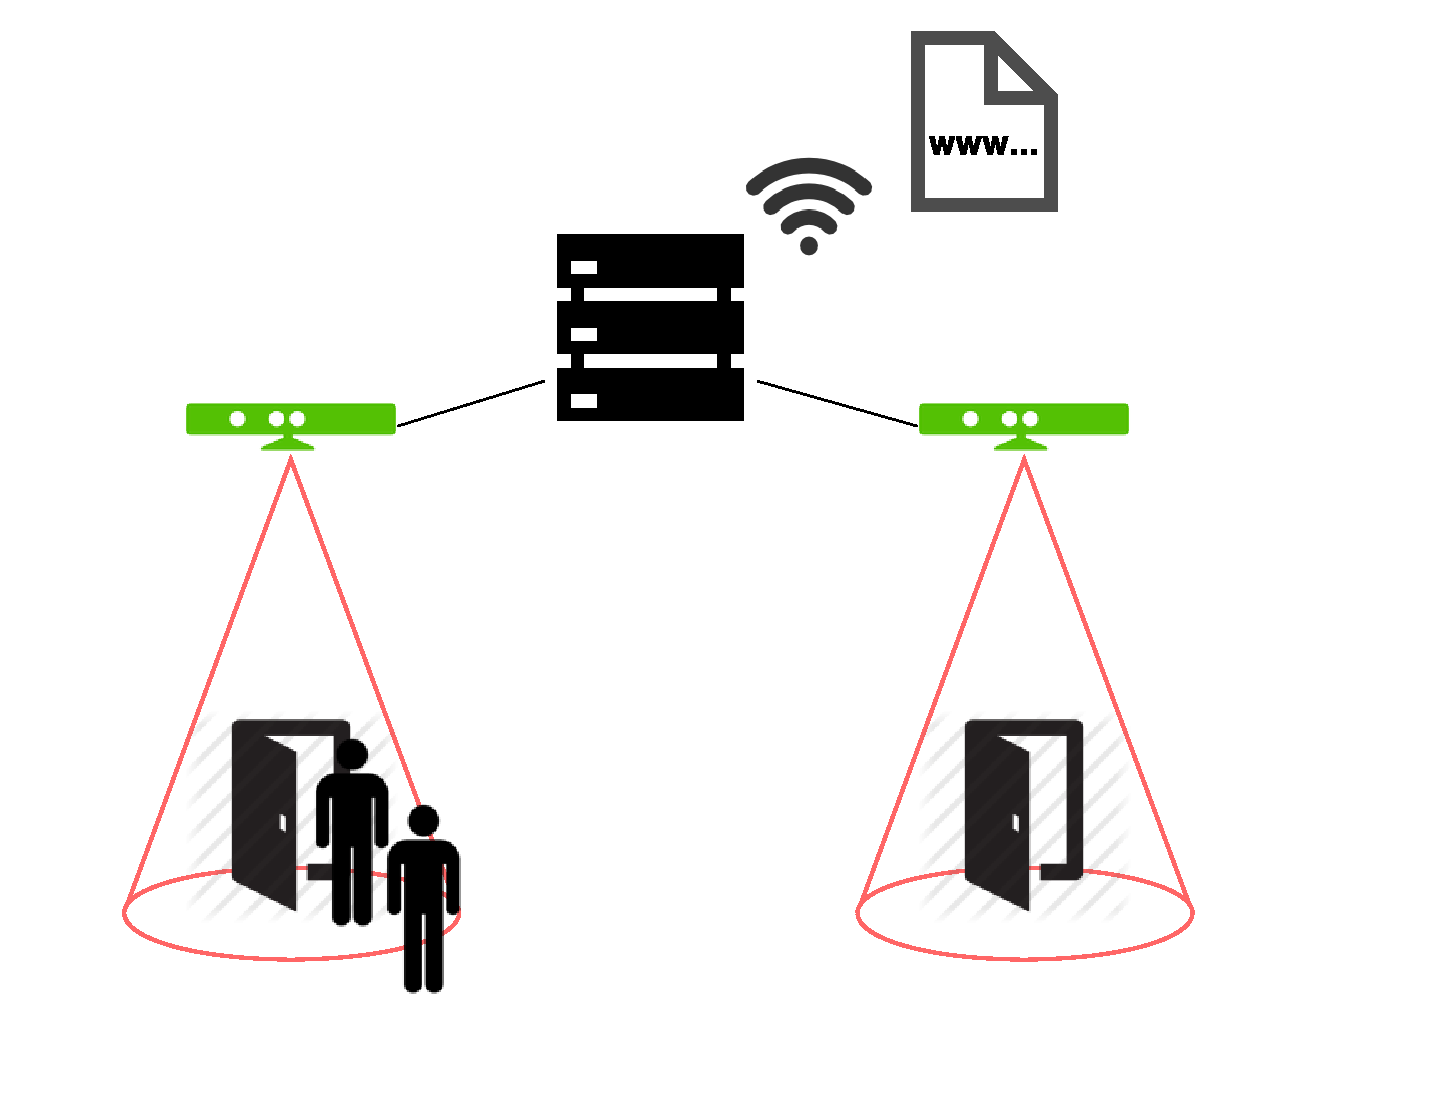
\includegraphics[width=\linewidth]{images/system_overview.pdf}
	\caption[Overview system setup]{\textit{A figure depicting the system, with a sensor mounted above each room entrance.}}
	\label{fig:system_overview}  %Skapar referens till figuren
\end{figure}

\subsection{Sensor placement}
Where do i mount kinect? 


\newpage
\section{The User Interface}
\label{sec:evaluation}
Text about the UI and result presentation.


\subsection{Presentation of results}
Text here

\subsection{Webpage}
Text here



\newpage
\section{Configuring the System}
\label{sec:current_pipeline}
This section describes how to tune the system using the GUI.










\end{document}
